\documentclass[letterpaper, 10 pt, conference]{ieeeconf} 
\IEEEoverridecommandlockouts                       
\overrideIEEEmargins
\usepackage[utf8]{inputenc}
\usepackage[T1]{fontenc}
\usepackage{graphicx}
\usepackage{array}
\usepackage{subcaption}
\captionsetup{compatibility=false}
\usepackage{cuted}%
\usepackage{afterpage}%


\title{
		\usefont{OT1}{bch}{b}{n}
		\normalfont \normalsize \textsc{2022 FALL SEMESTER, INTRODUCTION TO DATA SCIENCE - CSE0473}\\ [18pt]
		\huge Shopping Exprience Through Explainable\\Artificial Intelligence \\

}

\usepackage{authblk}
\author{Nasibullah Qarizada \\ 1900004691@stu.iku.edu.tr}
\begin{document}

\maketitle

\begin{strip}
\begin{abstract}

The huge increase of technology affected traditional retail shopping or well known as brick-and-mortar shopping experience with involution of digitalized systems like Augmented Reality. Undoubtedly, all these implementations are done to simplify the procedure of shopping and present information to customers in easy and luxury ways. however, the incomes might not be expected as estimated. Therefore, today we analyze the impacts of augmented reality and artificial intelligence with personalized shopping assistant application on shopping experience.
\\Approach: The research is done by analyzing a survey done with 252 participants, containing questions regarding to different shopping scenarios and expected their reviews.
\\Findings: To summarize the results of the survey, it has been proved the “Augmented reality” or “Explainable AI and Augmented Reality” are having a positive impact on shopping experience.
\\Keywords: Shopping, Augmented Reality, Explainable Artificial Intelligence Augmented Reality, Digitalizing, Brick-and-Mortar, Digital Shopping Assistant.\\\\

\end{abstract}
\end{strip}

%%%%%%%%%%%%%%%%%%%%%%%%%%%%%%%%%%%%%%%%%%%%%%%%%%%%%%%%%%%%%%%%%%%%%%%%%%%%%%%%

\section{INTRODUCTION}

Technology is anywhere in our nowadays life. As it always been, the main target is to make the life easier as possible. Due the huge rise of technology, the ideas of using it in our daily lives are also increasing. Specially after the Covid-19 pandemic years and decrease in sales, one of the recent goals of mankind is to involve technology with our traditional shopping habit. The retailers were supposed to know the reason and a solution to these kinds of problems and furthermore, to provide a better way of shopping  to customers. In these situations, one of the charming ideas was usage of Augmented Reality and Artificial Intelligence in shopping. In other words, the product information (Comparison, Discounts, Recommendations) and photos were delivered to customers through their phone. it was providing personalization and interactivity  This system also thought that it would motivate customers to buy more products, positively effect customer behaviors and to avoid physical contact with selling assistants during Covid-19.\\ 
However, usage of such technologies without being assure might be financially hard. It has also potential to make the company to lose lots of their customers. Therefore,  best way to get assure of such attempts is to start a survey with your customers, ask them questions or provide a demo.\\
This research will also be containing the results of a survey done, to find out the results of usage of RSS(Regular Shopping Scenario), ARSS(Augmented Reality Shopping Scenario) and EARSS(Explainable Augmented Reality Shopping Scenario). The dataset is gathered by participation and answering of 252 participants, which has gradable and reviewable parts for any Shopping Scenarios (RSS, ARSS and EARSS). Which in this report the results have been analyzed from different perspectives to gain a general knowledge on usage of such technologies.\\
The paper is structured as follows: Section 1: Introduction to concept and research goals, Section 2: The background of study and previous works, Section 3: Expanded explanation of methodologies and strategies used. Section 4: Results of the research. Section 5: Conclusion.


\section{BACKGROUND AND PREVIOUS WORKS}
In this part, the previous and related works done in such fields are mentioned. It is good to underline that their works and research contributed a lot in developing this research. Furthermore, at the end of the part there would be the background of my research, which contains the limitations, the hypothesis and overall summarization. 



\subsection{Related Works}

Alongside the newness of the usage of digitalized systems in shopping, there are some several research according to the effectiveness of such systems. In a research$^1$ done by Peter C. Verhoef at University of Groningen, He analysis the different ways of reaching retailers to customers, through their mobile phone and social media. This habit leads us to a new term multi-channel retailing. Surprisingly, the results are expectedly good. At another research$^2$ done by Salvatore Parise in Babson college, analysis the importance and effects of personalized advertisements and information. Implementation of such ability to any shopping system make retailers to decide sharp about their promotion or shopping discussions. Alongside, a very seemingly research$^3$ done by Virginie Lavoie also analysis the customers reflexes and behaviors to Augmented Reality in retails. As a conclusion of these research the implementation of Augmented Reality, Explainable AI features or personalized information has been resulted positively yet. Today, we would be having a closer look to its affects and analyze with perspective of several participants.

\subsection{Conceptual Background}

As mentioned in introduction part in this research, It will be comparing effectiveness of three different shopping scenarios. They are divided into two categories, Assisted and Unassisted. Let us have a closer look.\\
Regular Shopping Scenario: Also known as RSS. This is the traditional method of shopping which will be done between a shopping assistant and a buyer. It is counted as unassisted shopping system.\\
Augmented Reality Shopping Scenario: Also known as ARSS or Assisted shopping. In this type, users will start their experience with downloading an Android-based application. As you see in figure[1],Figure[2] and Figure[3] The application will be showing the products information or buttons such as adding to basket or buying them.
\begin{figure}[!ht]
    \centering
    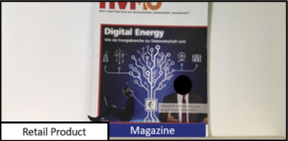
\includegraphics{Picture1.png}
    \caption{Application Scanning Screen}
\end{figure}
\begin{figure}[!ht]
    \centering
    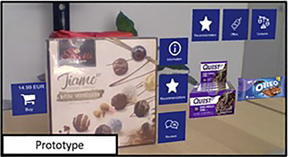
\includegraphics{Picture2.png}
    \caption{Product Alternatives}
\end{figure}
\begin{figure}[!ht]
    \centering
    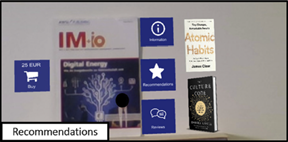
\includegraphics{Picture3.png}
    \caption{Product Alternatives}
\end{figure}
Explainable Artificial Intelligence Augmented Reality Shopping Scenario: Also known as EARSS, which is also assisted shopping type. The idea is accurately same with Augmented Reality Shopping Scenario but in this concept artificial intelligence is also used. Now, the users can see personalized product recommendations, product comparisons and product information. Shown in Figure[4] and Figure[5]\\
\begin{figure}[!ht]
    \centering
    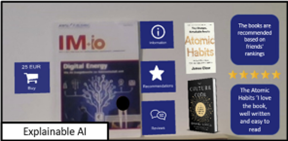
\includegraphics{Picture4.png}
    \caption{Product Information}
\end{figure}\\
\begin{figure}[!ht]
    \centering
    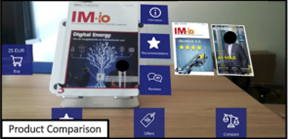
\includegraphics{Picture5.png}
    \caption{Product Information}
\end{figure}\\


\subsubsection{Hypothesis}\hfill\\\hfill\\
h1: EARSS and ARSS is preferred a lot in terms of usability than RSS \\
h2: EARSS and ARSS is preferred a lot in terms of entertainment than RSS \\
h3: EARSS and ARSS is preferred a lot in terms of informativity than RSS \\
h4: EARSS and ARSS is preferred a lot in terms of irritability than RSS \\
h5: EARSS and ARSS is encouraged customers to have a higher purchase intention than RSS.\\
h6: EARSS is much more trust worthy than ARSS.\\
The detailed and visualized table of our contents and datasets are also sketched in figure[1]\\

\subsubsection{Limitations}\hfill\\\hfill\\
Augmented Reality and artificial intelligence are placed at the top of trending list of technological equipments. Reaching a sharp result in such field analyses might be requiring a huge amount of dataset. Our dataset might not be the reason gain a sharp result but surely, it would help us to have an idea in case of effectiveness of mentioned systems.\\

\section{METHODOLOGY}
This chapter would describe the methods and strategies done to gain the specified hypothesis and results such as Data preprocessing, Feature Engineering, statistical analysis, statistical test, or other strategies to make the dataset to perform an acceptable accuracy. \\
Dataset: Before involving to development part, gaining idea about conclusion of dataset increases the effectiveness of research and helps to catch analysis from different perspectives. To have a closer look, the participants were decided about 6 aspects for each of three shopping scenarios. Here in figure[6] you see all categories and fields that the questions has been asked from participants.

\begin{figure}[!ht]
    \centering
    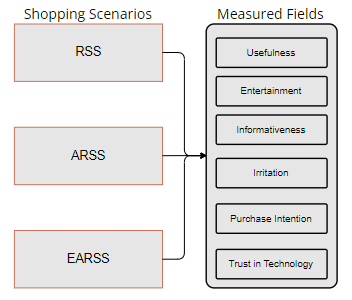
\includegraphics[scale = 0.6]{Picture6.png}
    \caption{Dataset Road-map}
    
\end{figure}

\subsection{Design and Structure:}
While approaching the statistics and results for this research, we passed through some process. As mentioned in figure[7] Fetching data, Pre-processing, Test Analysis, visualization, and testing are the main parts of this process. This subtitle would be describing the steps and explanations while doing the mentioned processes.\\


\begin{figure}[!ht]
    \centering
    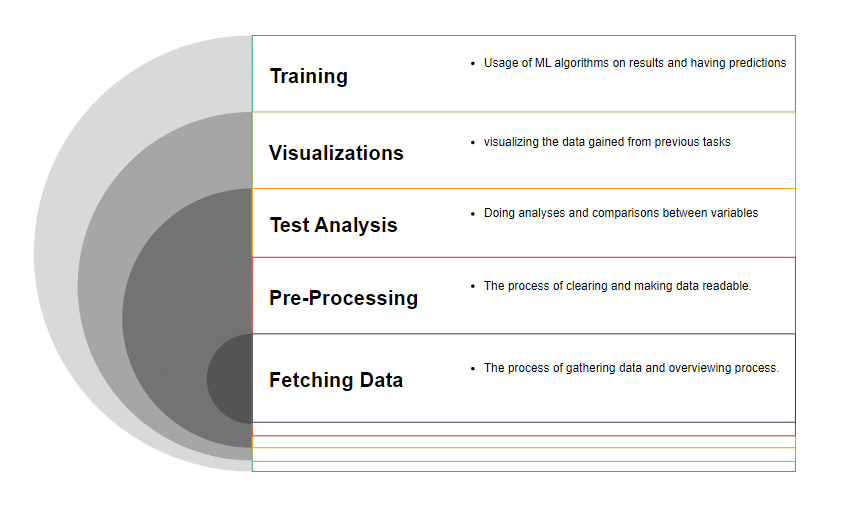
\includegraphics[scale = 0.4]{Picture7.png}
    \caption{Road-map}
    
\end{figure}



\subsubsection{Fetching Dataset}\hfill\\

Alongside the dataset given was ready to extract but there were some points which needed maintenance. In some SPSS and recalculated columns (Ex, Gender SPSS, Total Usefulness – RSS and etc.), huge amount of data was missing. The required data has been recalculated and verified by specified calculation steps. Furthermore, before entering the pre-processing section some empty columns has been deleted manually in case to reduce the complexity of dataset while doing first analysis and to have an overall sense to dataset.\\

\subsubsection{Pre-Processing}\hfill\\

This part is underlined as one of the most important parts in Data Science. It is usually done to interpret and use the data easier. Therefore, there are several ways and methods to perform to do it. Some of the pre-processing methods used while doing this research are removing unused columns, lower casing all words, removing punctuation, removing stop words, removing multiple spaces. Furthermore, in some parts of data analysis I applied the Standardization, Normalization, Tokenization, Vectorization, and one-hot coding  processes which helps on analyzing and sorting data.\\

\subsubsection{Text Analysis}\hfill\\

Test Analysis: In test analysis as first step it is used to visualize and check the results and do the comparison between variable or columns by measuring the metrics, testing the scope. The Test part is to mainly there to confirm and shed a led on these results. There are several methods for reaching to these results. Exploratory data analysis, regression and classification, forecasting and data grouping are included also in this section. All of them are preferred for a specific field of testing. Confirmation of hypothesis (mentioned in conceptual background part) will also be accepted or rejected in this part.\\

\subsubsection{Visualization}\hfill\\

The gathered and confirmed scores, the data gained from the dataset will be visualized and presented by developing matplotlib, seaborn and some other python visualization libraries. The main goal of this part is to deliver the results of research and performed tests to readers by applying attractive and simple visualization methods.\\

\subsubsection{Training}\hfill\\

Training part is based on machine learning algorithms. Main goal of machine learning is to allow users or software to become more accurate at predicting future of the given data. To reach those predictions there are several algorithms, mainly divided into two categories. Supervised and Unsupervised. Supervised algorithms use labeled dataset meanwhile unsupervised algorithms are in chase of analyzing and clustering unlabeled datasets. Supervised algorithms are separated in two parts classification and regression. Alongside, Unsupervised algorithms are generally divided into three, Clustering, Association, and dimensionality. The algorithms used in this research are Random Forest, Naïve Bayes, Decision tree, Logistic Regression, SVM algorithm. (This part might be edited on upcoming steps.)

\section{RESULTS}

\subsection{Participants}

The survey was shared online with the participants and the first part of supposed to be filled with participants personal information. Germany, Austria and USA were the participants living countries. The figure[8] is list of top 10 cities which most of the participants joined to the survey. Berlin, Vienna, and Hamburg had the most participants as shown in figure[8] \\

\begin{figure}[!ht]
    \centering
    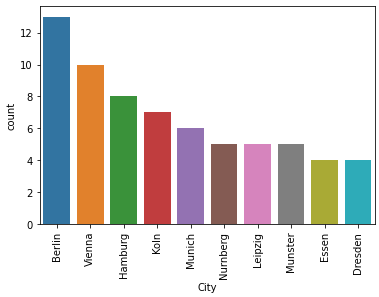
\includegraphics[scale = 0.8]{Picture8.png}
    \caption{Participants' Cities}
\end{figure}

The average of participants’ age was 37. As shown in figure[9], I decided to represent them in categorized way. Table[1] represents number of participants from each group. \\

\begin{table}[!ht]
\begin{tabular}{ | m{4cm} | m{3.8cm}| }
\hline
Age Group & Participants \\ \hline
18 to 27  & 64           \\ \hline
28 to 37  & 70           \\ \hline
38 to 47  & 66           \\ \hline
48 to 57  & 36           \\ \hline
58 to 67  & 14           \\ \hline
68 to 100 & 1            \\ \hline
\end{tabular}
\caption{\label{table}Age Groups}
\end{table}

\begin{figure}[!ht]
    \centering
    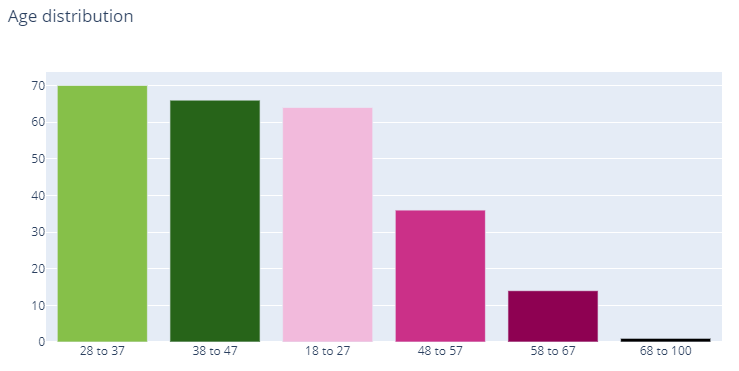
\includegraphics[width = 9cm, height = 5cm]{Picture9.png}
    \caption{Age Groups}
\end{figure}


Among these values 46.8\% (118) of them were male, 52.4\% (132) of them were female and 0.79\% (2) of them defined there genders as diverse. The figure[10] represent the visualized range of this part.


\begin{figure}[!ht]
    \centering
    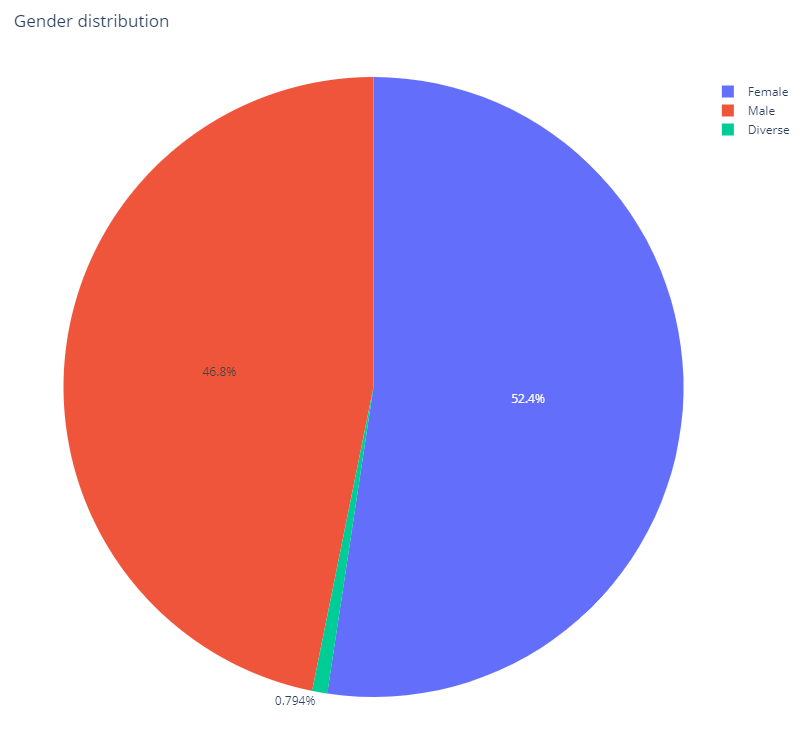
\includegraphics[scale = 0.3]{Picture10.png}
    \caption{Genders}
\end{figure}

Now to check the frequency of shopping of participants in last 30 days the figure[11] helps us to understand the range. %In table[II] you can see the detailed values of each variable.

%\begin{table}[!ht]
%\begin{tabular}{ | m{4cm} | m{3.8cm}| }
%\hline
%Frequency              & Participants  \\ 
%\hline
%Moderately Frequently~ & 115           \\ 
%\hline
%Slightly Frequently    & 63            \\ 
%\hline
%Very Frequently        & 42            \\ 
%\hline
%Not at all Frequently  & 25            \\ 
%\hline
%Extremely Frequently   & 7             \\
%\hline
%\end{tabular}
%\caption{\label{demo-table}Shopping Frequency}
%\end{table}

\begin{figure}[!ht]
    \centering
    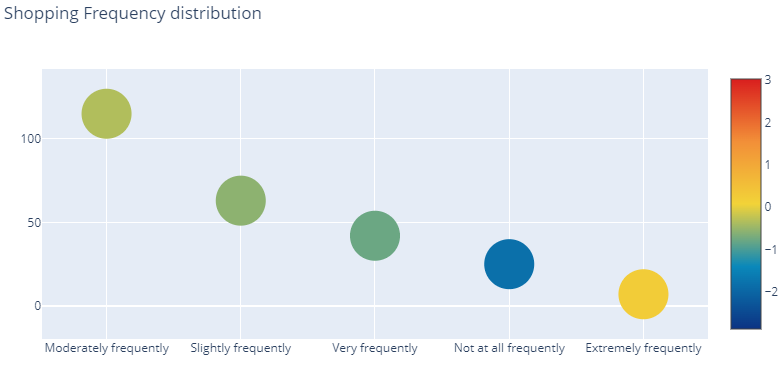
\includegraphics[width = 8cm, height = 4.5cm]{Picture11.png}
    \caption{Shopping Frequency In last 30 Days}
\end{figure}


Figure[12] represents the education level our participants. It is good to note that the expected knowledge level from our participants is accurately high since a huge part of them graduated from university, masters, or doctorate. \\

\begin{figure}[!ht]
    \centering
    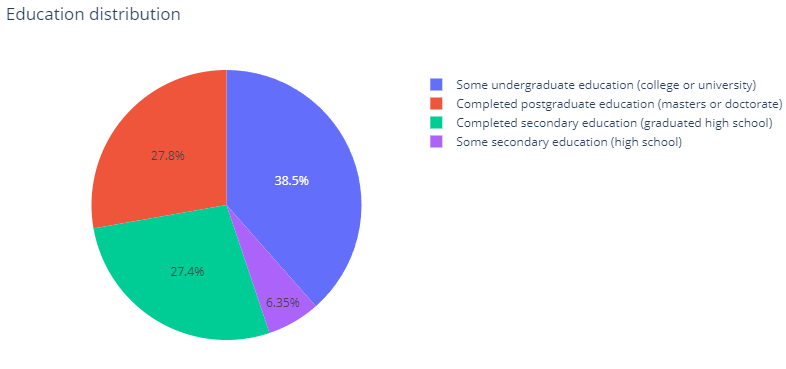
\includegraphics[scale = 0.4]{Picture12.png}
    \caption{Participant's Education Level}
\end{figure}

Figure[13] is representing the average of monthly income of participants. To have some sharp information on this case, table[III] is filled with detailed information gathered from this chart.
   

\begin{table}[!ht]
\begin{tabular}{ | m{4cm} | m{3.8cm}| }
\hline
Average Income  & Participants  \\ 
\hline
1000€           & 63 (25\%)     \\ 
\hline
1000€ and 2000€ & 85 (33.7\%)   \\ 
\hline
2000€ and 3000€ & 53 (21\%)     \\ 
\hline
3000€ and 4000€ & 29 (11.5\%)   \\ 
\hline
4000€ and 5000€ & 15 (6\%)      \\ 
\hline
5000€ and above & 7 (2.8\%)     \\
\hline
\end{tabular}
\caption{\label{demo-table}Monthly Income}
\end{table}


\begin{figure}[!ht]
    \centering
    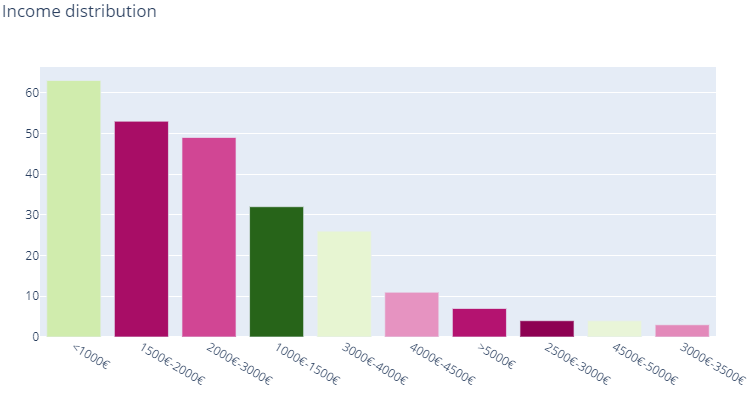
\includegraphics[scale = 0.4]{Picture13.png}
    \caption{Categorized Monthly Income}
\end{figure}

\subsection{Statistical Analysis}
Statistical Analysis: Now, it’s time to get to the main point of research. In this part we are checking the results of statistical analysis. Figure[17]is list of all scenarios and measured aspects. As shown, different questions asked from each aspect. According to the answer of participants the mean values and standard deviation of each aspect is shared.\\
Figure[14] and Figure[15] shows the weight points of participants choices according to their age and our three different shopping scenarios. In RSS we see that the average of participants votes is around 2.95 but it is good to notice in ARSS and EARSS (Figure[14] and Figure[15]) this amount is increased to 3.05 in both.\\
As mentioned in H6, we hypothesized that with the increase of age, ratio of selection of ARSS and EARSS is decreasing. It is estimated that usage of these technological assets might be hard to use by older people which the consequences might be the failure of gadgets or countable decreases in shopping field.  \\ As first step of test analysis part we have to analyze the distribution of our data. Before checking distribution, it is suggested to analyze the skewness of data to gain some overall information. As shown in figure [Figure Number] it is saying whether our data is positively, negatively, or symmetrically skewed. 

\begin{figure}[!ht]
    \centering
    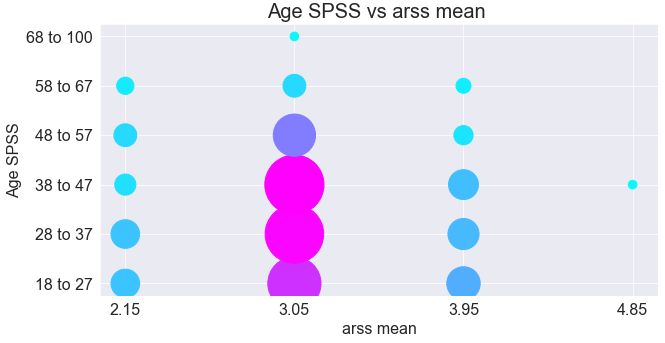
\includegraphics[scale = 0.5]{Picture14.png}
    \caption{ARSS vs Ages}
\end{figure}

\begin{figure}[!ht]
    \centering
    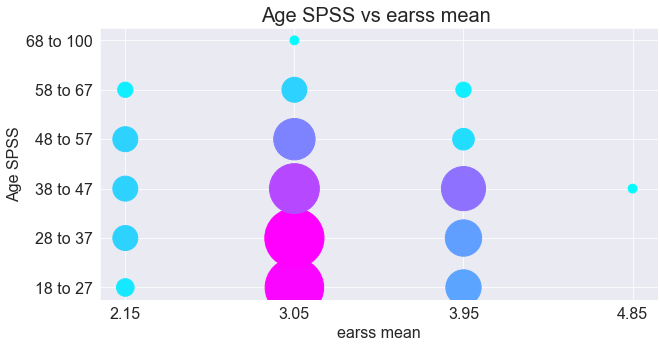
\includegraphics[scale = 0.5]{Picture15.png}
    \caption{EARSS vs Ages}
\end{figure}
In figures [20. 21, 22, 23, 24 and 25] the distribution of data in RSS has visualized. in case of normality distribution we can say that our data is only distributed normally in Figure[21] or column of total enjoyment - RSS. meanwhile, fourth of them negatively negative skewed except Total irritation - RSS column.\\

\pagebreak

\begin{figure}[!ht]
    \centering
    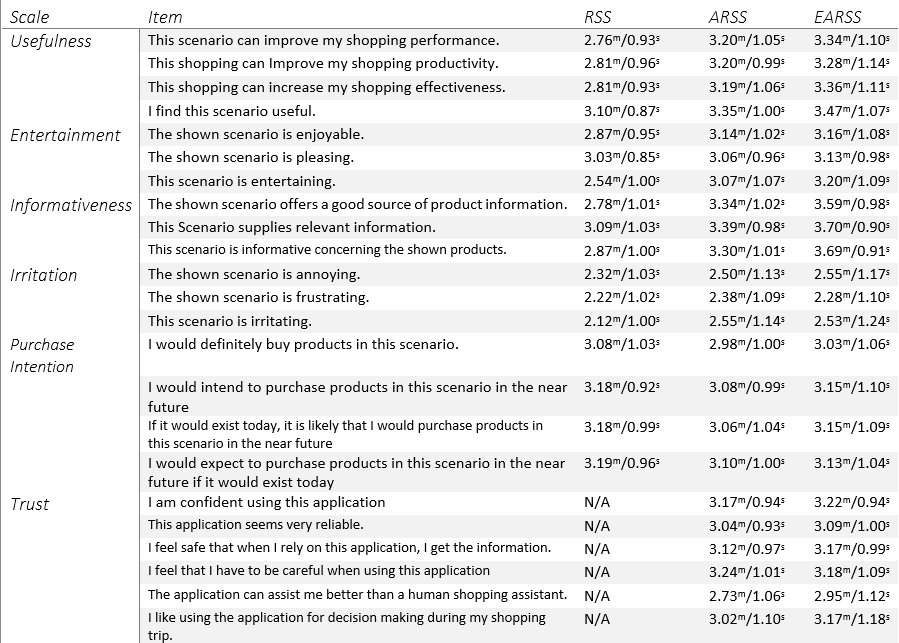
\includegraphics[scale = 0.7]{Picture17.png}
    \caption{Main Differences and Standard Deviation}
\end{figure}


\begin{strip}
    \\\\\\\\\\\\\\\\\\\\\\\\\\\\\\\\\\\\\\Before testing analysis, Figure[16] represents the Mean Values and Standard Deviation for each given scenario in different fields including, Usefulness, Entertainment, Informativeness, Irritation, Purchase Intention and Trust. To compare them with given values, In Usefulness case RSS has 2.87, ARSS has 3.24 and EARSS has 3.36. In Entertainment RSS has 2.81, ARSS has 3.09 and EARSS is 3.36. In being Informativeness RSS has 2.92, ARSS has 3.35 and EARSS has 3.66. In Irritation RSS has 2.92, ARSS has 2.48 and EARSS has 2.45. And finally in total purchase intention RSS has 3.16, ARSS has 3.05 and EARSS has 3.12. before contributing to testing concepts, we saw that at first 4 category ARSS and EARSS were having a high range of mean than RSS. But  in Purchase Intention participants were preferred to do shopping regularly. To compare trust between ARSS and EARSS. EARSS is having 3.13 mean range meanwhile ARSS is 3.05. So far, it is proved that h1, h2, h3, h4 and h6 were true except H5. After normality analysis and correlation analysis and doing specific test according to our data we would jump to statistical test in parametric and non-parametric format. therefore, we can confirm our hypothesis according to the results gained. \\\\\\\\\\\\\\\\\\\\
\end{strip}



\pagebreak
\newlength{\common}
\begin{figure}[!ht]
\settoheight{\common}{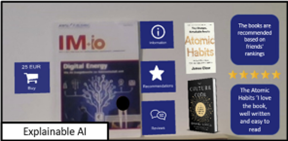
\includegraphics[width=.3\textwidth]{Picture4.png}}% get height
\subfloat[Figure 20]{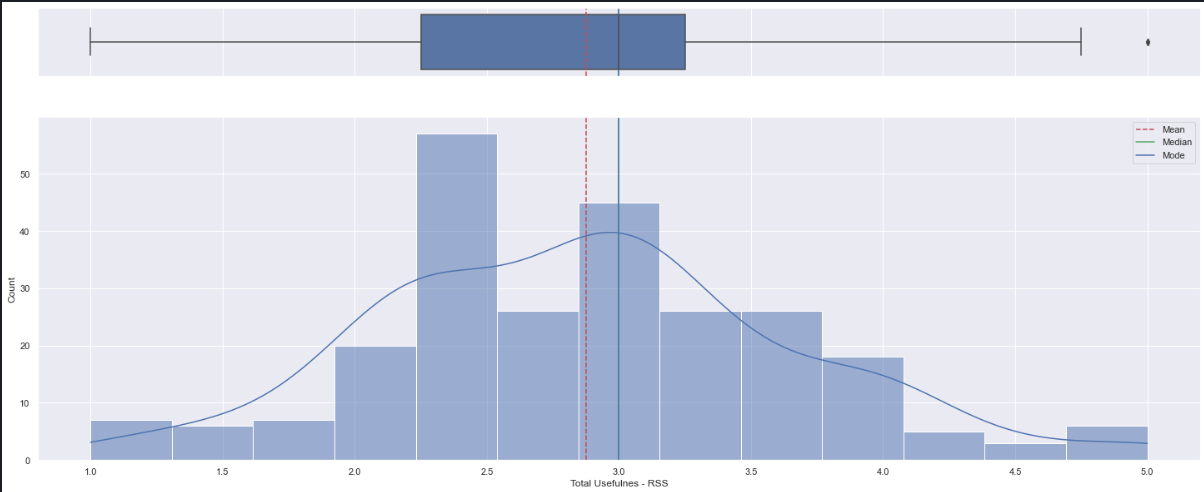
\includegraphics[scale = 0.25]{rss_usefulnes.png}}\hfill
\subfloat[Figure 21]{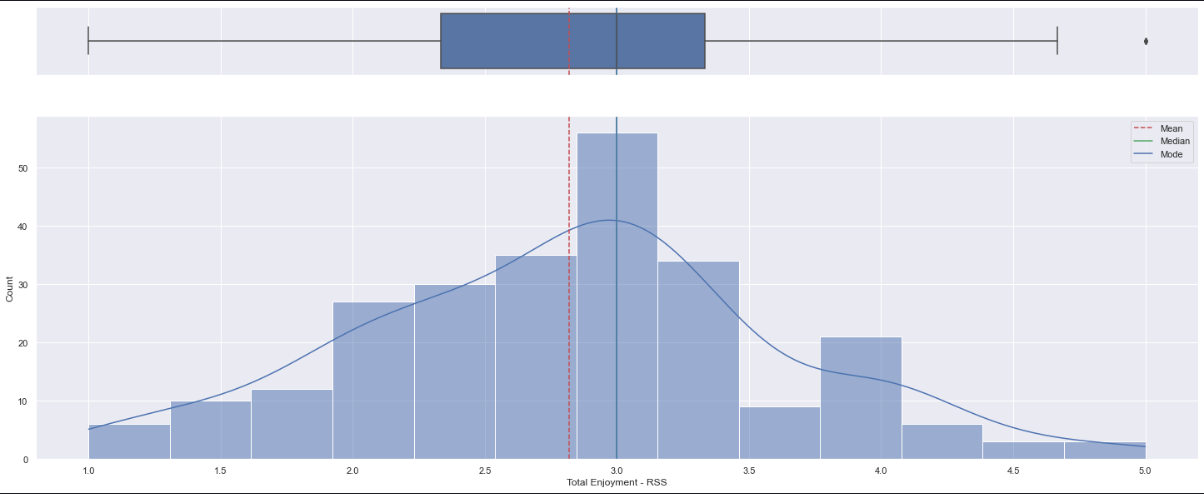
\includegraphics[scale = 0.25]{rss_enjoyment.png}}\hfill
\subfloat[Figure 22]{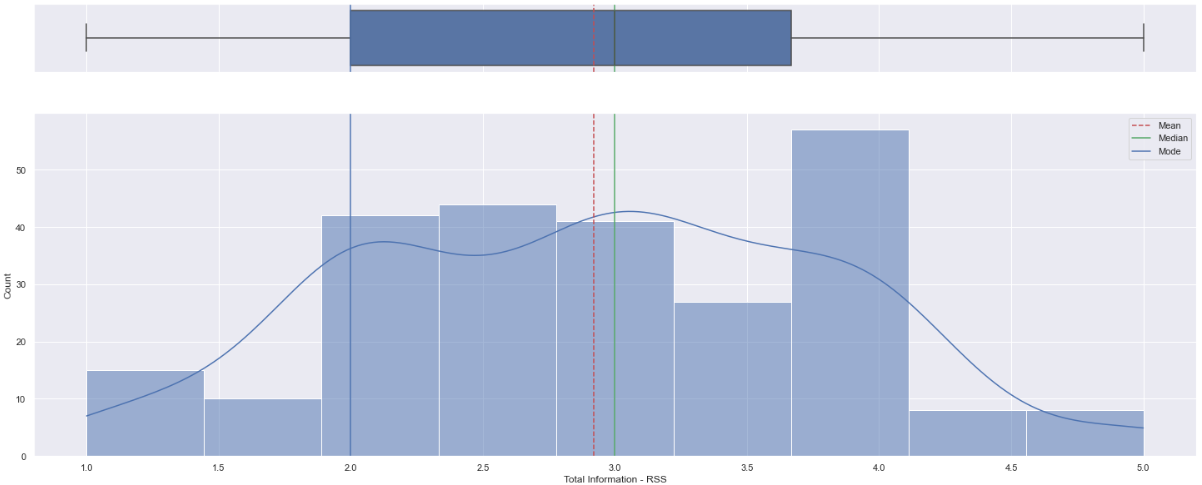
\includegraphics[scale = 0.25]{rss_information.png}}\hfill
\subfloat[Figure 23]{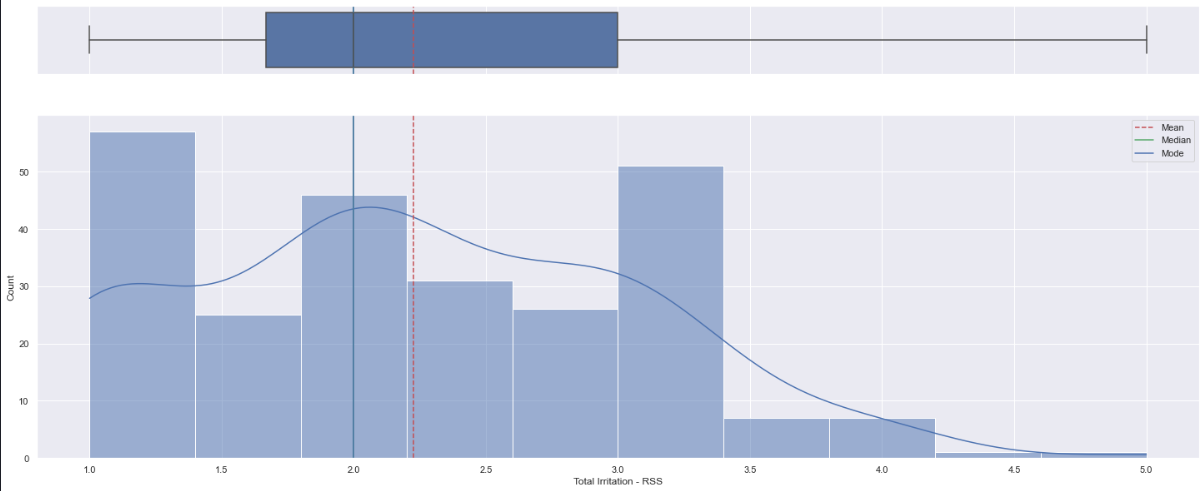
\includegraphics[scale = 0.25]{rss_irritation.png}}\hfill
\subfloat[Figure 24]{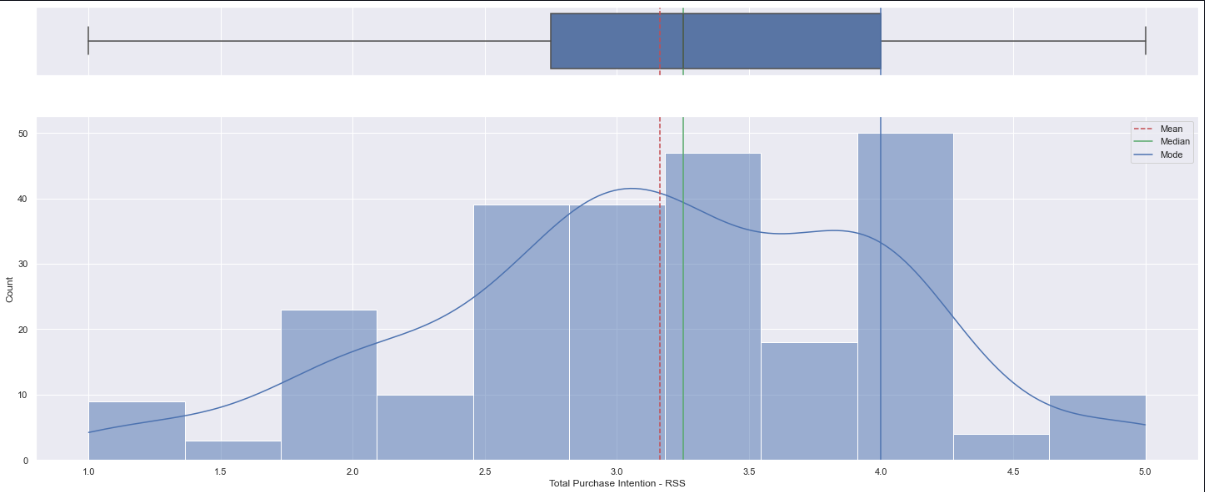
\includegraphics[scale = 0.25]{rss_purchase_intention.png}}
\end{figure}


In figures [25, 26, 27, 28, 29 and 30] the distribution of data in ARSS has visualized. in case of normality distribution we can say that our data is not distributed normally. meanwhile, four of columns were positively skewed except column total usefulness.

\begin{figure}[!ht]
\settoheight{\common}{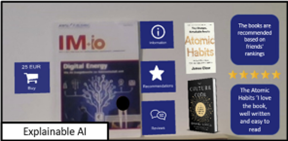
\includegraphics[width=.3\textwidth]{Picture4.png}}% get height
\subfloat[Figure 25]{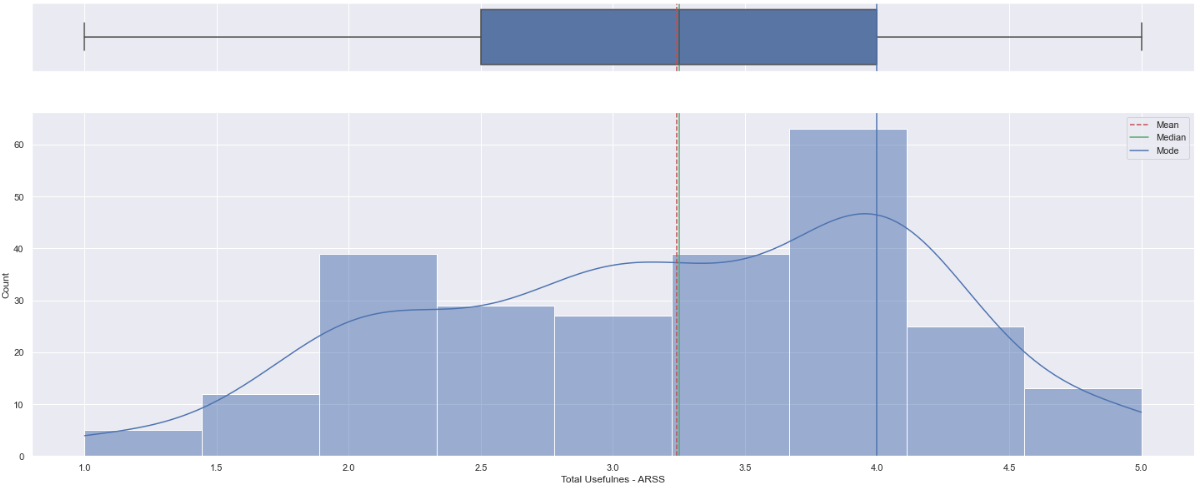
\includegraphics[scale = 0.25]{arss_usefulnes.png}}\hfill
\subfloat[Figure 26]{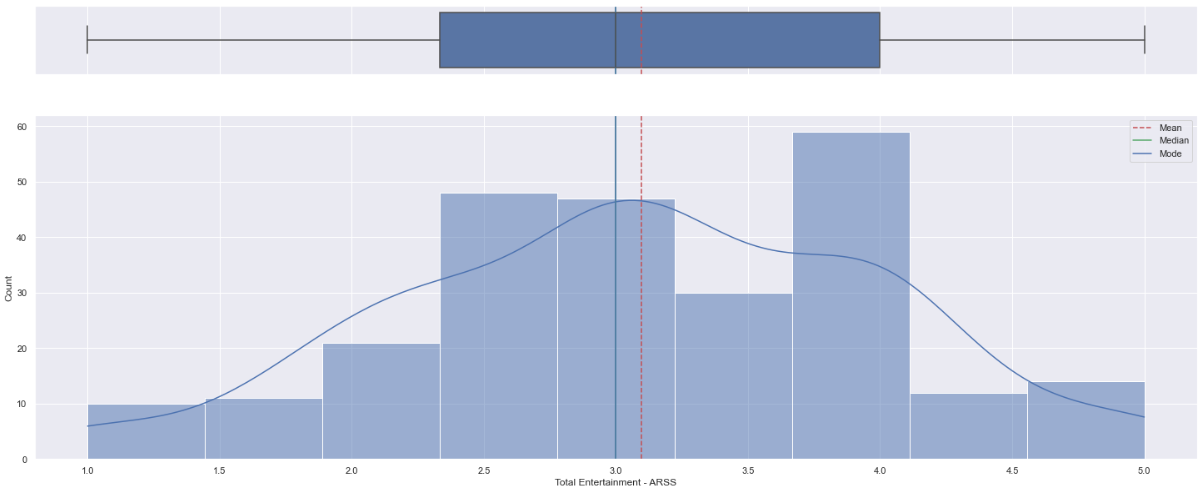
\includegraphics[scale = 0.25]{arss_enjoyment.png}}\hfill
\subfloat[Figure 27]{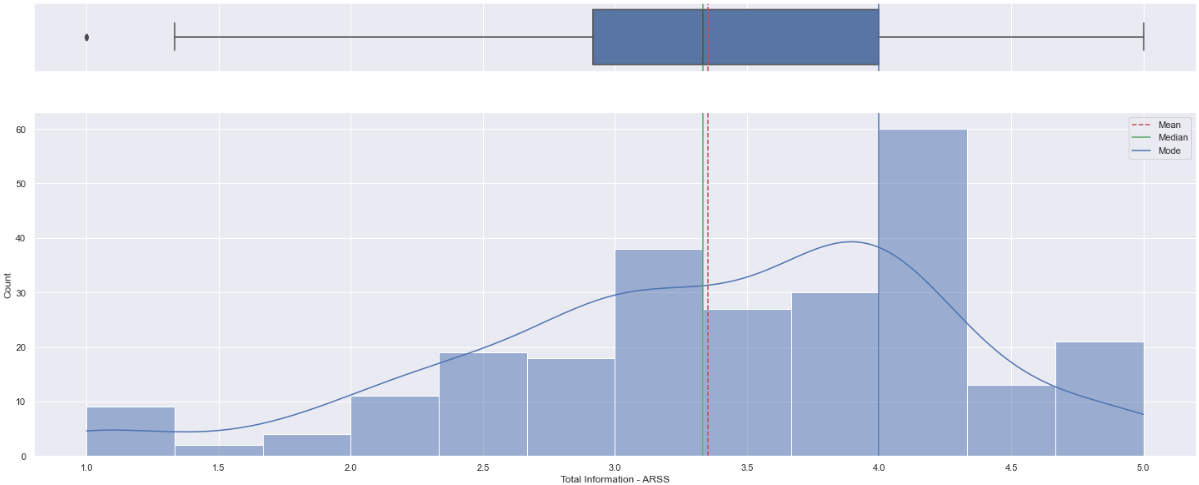
\includegraphics[scale = 0.25]{arss_information.png}}\hfill
\subfloat[Figure 28]{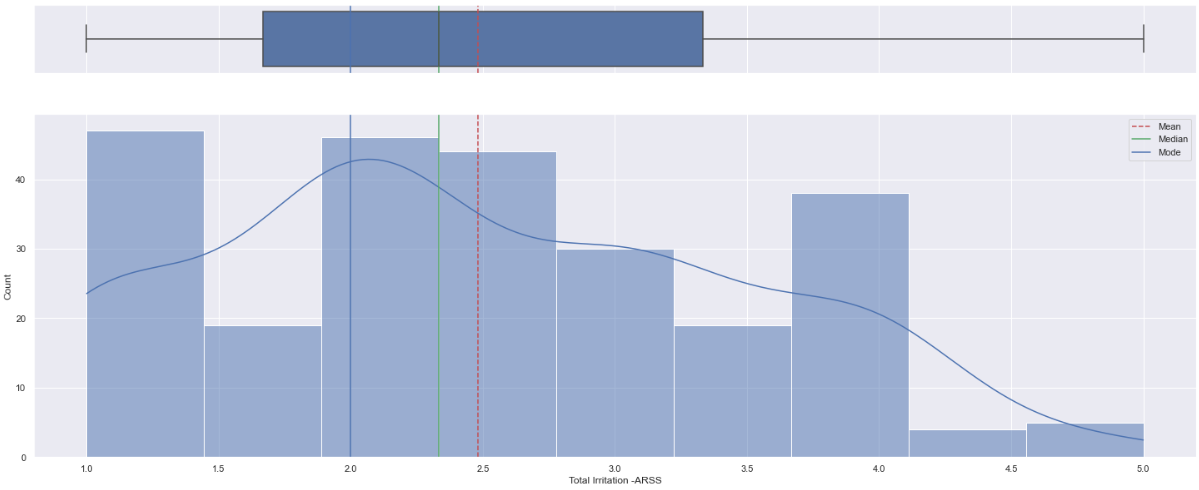
\includegraphics[scale = 0.25]{arss_irritation.png}}\hfill
\subfloat[Figure 29]{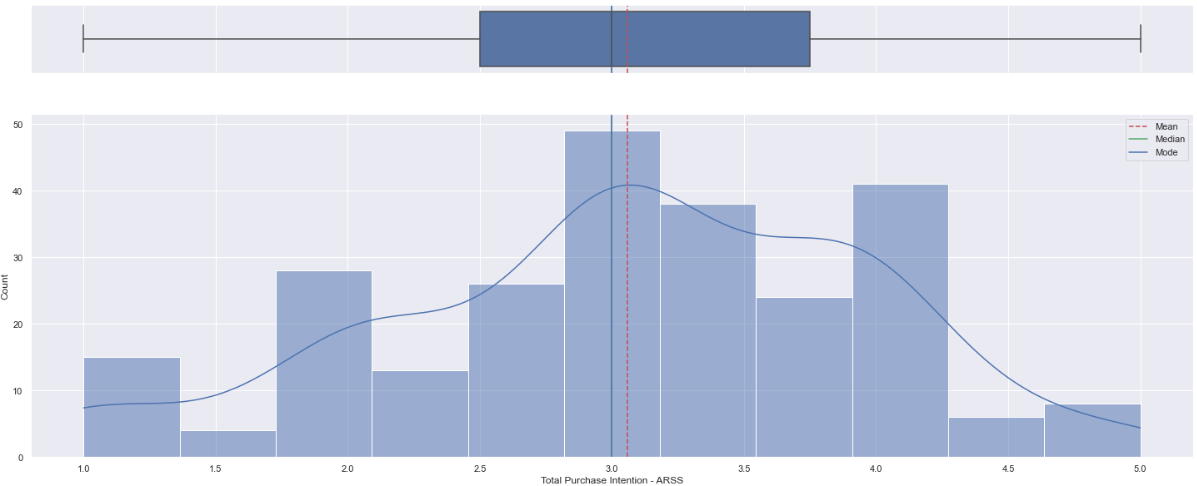
\includegraphics[scale = 0.25]{arss_purchase.png}}\hfill
\subfloat[Figure 30]{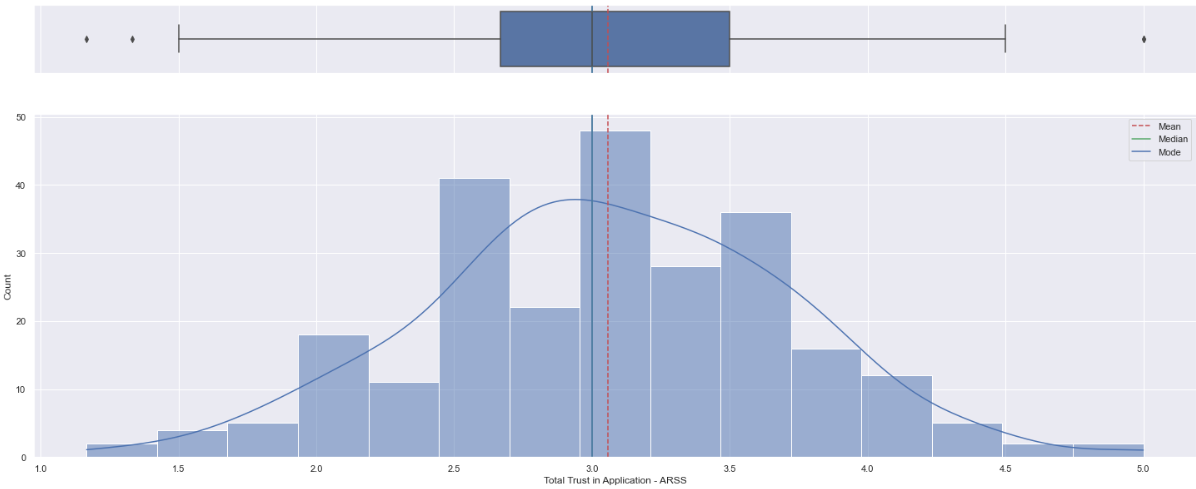
\includegraphics[scale = 0.25]{arss_trust.png}}
\end{figure}

In figures [31, 32, 33, 34, 35 and 36] the distribution of data in EARSS has visualized. in case of normality distribution we can say that none of our data is distributed normally. furthermore, Figure [31] is negatively skewed. meanwhile, the rest are negatively skewed.


\begin{figure}[!ht]
\settoheight{\common}{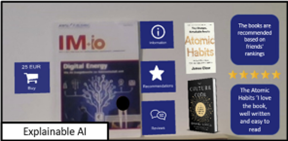
\includegraphics[width=.3\textwidth]{Picture4.png}}% get height
\subfloat[Figure 31]{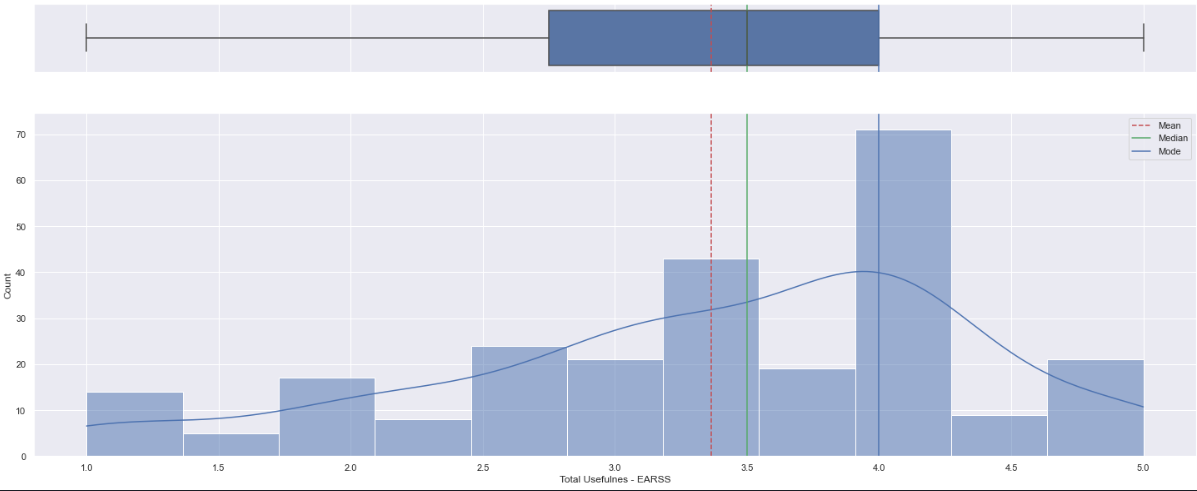
\includegraphics[scale = 0.25]{earss_usefulnes.png}}\hfill
\subfloat[Figure 32]{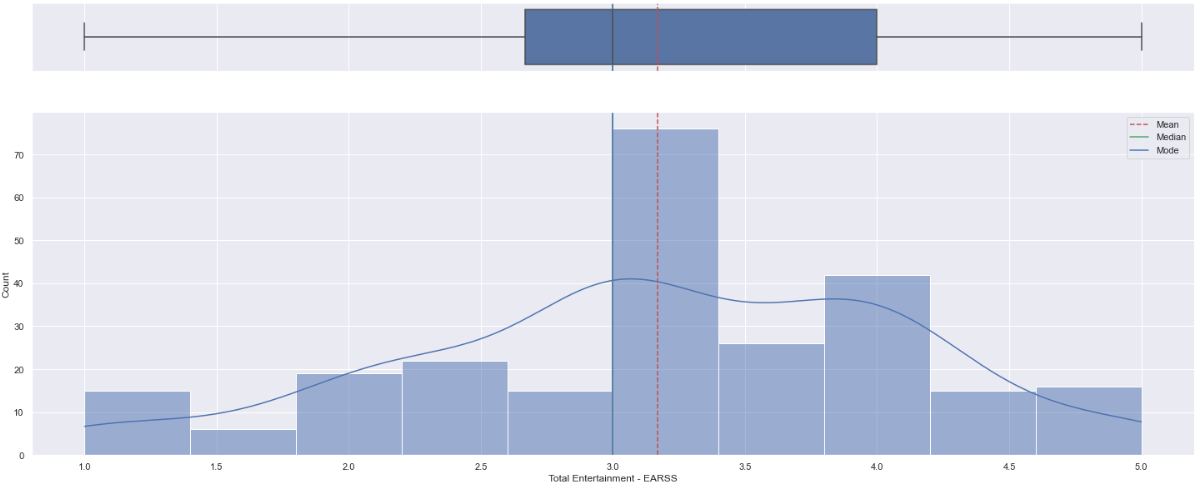
\includegraphics[scale = 0.25]{earss_enjoyment.png}}\hfill
\subfloat[Figure 33]{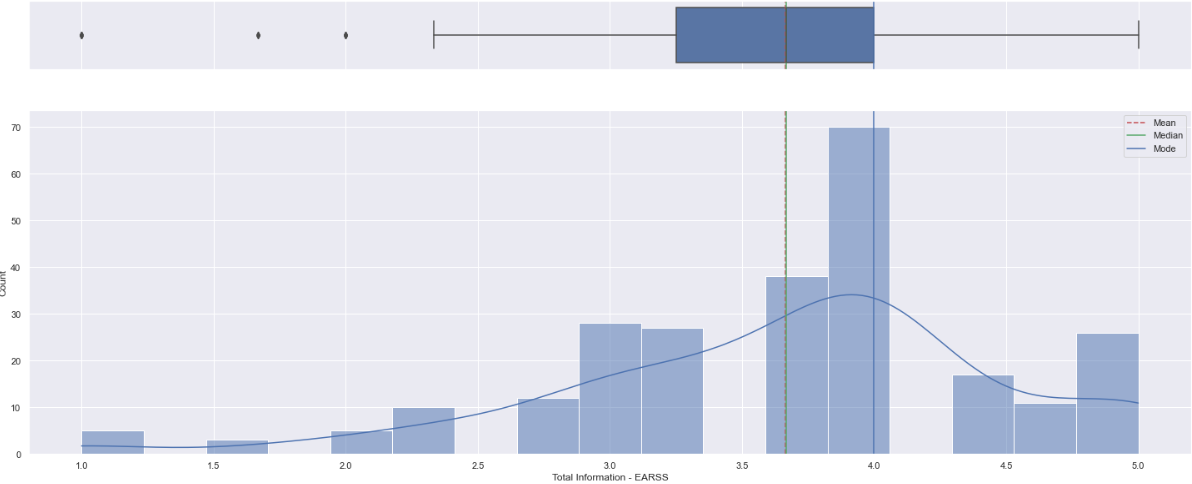
\includegraphics[scale = 0.25]{earss_information.png}}\hfill
\subfloat[Figure 34]{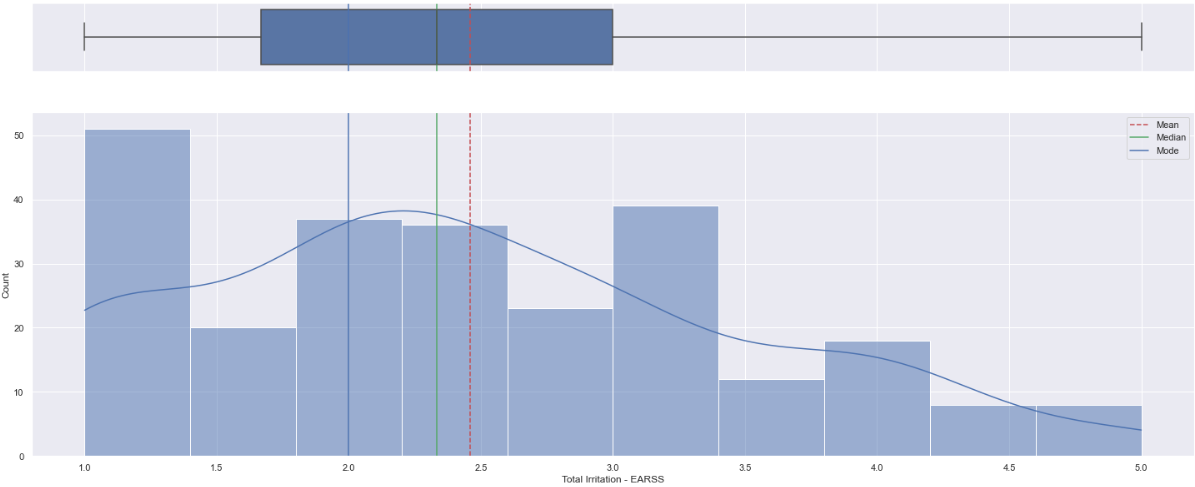
\includegraphics[scale = 0.25]{irritation_earss.png}}\hfill
\subfloat[Figure 35]{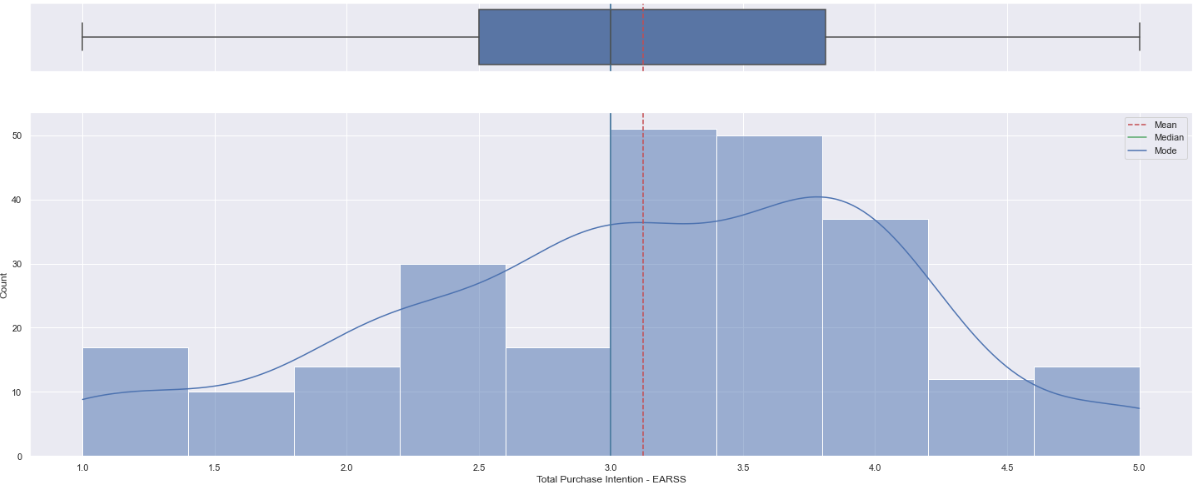
\includegraphics[scale = 0.25]{purchase_intention_earss.png}}\hfill
\subfloat[Figure 36]{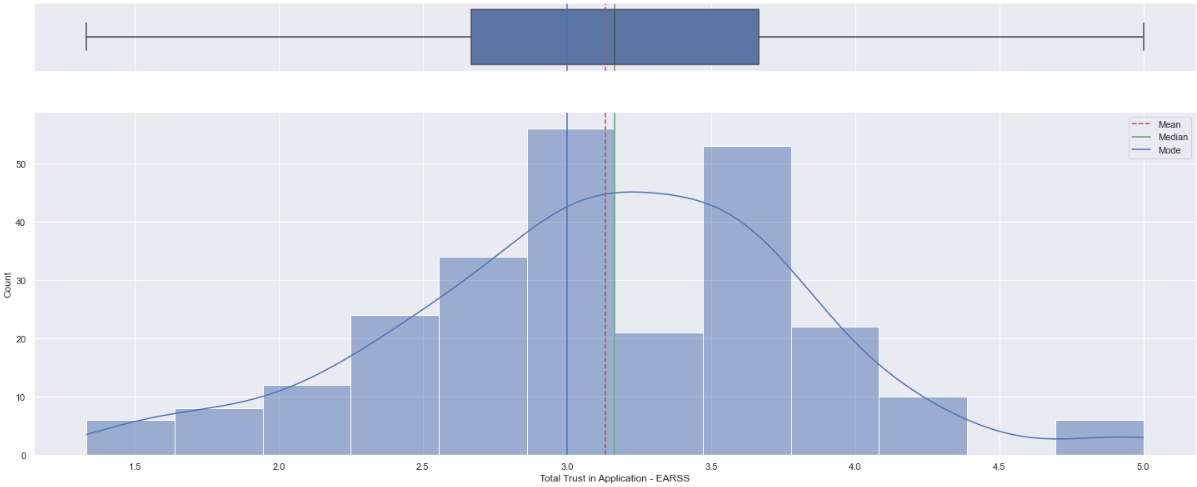
\includegraphics[scale = 0.25]{trust_earss.png}}
\end{figure}


\begin{figure}[h!]
\subsection{Normality tests}
It is usually done because based on the results it helps to decide on performing parametric or non-parametric tests. Table[III] is the list of plots of our data defining if they are normally distributed or not.
Furthermore, to get assure of normality results, there are several testing methods available. To confirm the results we gained from the Figures [20 to 36], we can start applying the mentioned normality tests. Anderson Darling, D’Agostino’s and Shapiro normality tests has been chosen for this research. Table [Table number] is the results of the tests. As shown third of tests compiled pretty closer results to each other, but since D’Agostino’s is widely used and preferred by most of the users previously our next decision would be on D’Agostino’s normality test. It is good to mention that significance level for these tests has been set to (P-value = 0.05).
\end{figure}


\begin{table}[h!]
\begin{tabular}{|l|l|l|l|l|}
\hline
                   &       & Anderson     & D'Agostino's & Shapiro \\ \hline
Usefulness         & RSS   & Not Gaussian & 0.201        & 0.001   \\ \hline
                   & ARSS  & Not Gaussian & 0.001        & 0.000   \\ \hline
                   & EARSS & Not Gaussian & 0.001        & 7.624   \\ \hline
Enjoyment          & RSS   & Not Gaussian & 0.868        & 0.000   \\ \hline
                   & ARSS  & Not Gaussian & 0.276        & 0.000   \\ \hline
                   & EARSS & Not Gaussian & 0.083        & 0.000   \\ \hline
Information        & RSS   & Not Gaussian & 0.029        & 0.000   \\ \hline
                   & ARSS  & Not Gaussian & 0.002        & 2.515   \\ \hline
                   & EARSS & Not Gaussian & 0.000        & 6.880   \\ \hline
Irritation         & RSS   & Not Gaussian & 0.025        & 3.45    \\ \hline
                   & ARSS  & Not Gaussian & 0.000        & 1.960   \\ \hline
                   & EARSS & Not Gaussian & 0.002        & 9.312   \\ \hline
Purchase Intention & RSS   & Not Gaussian & 0.232        & 0.000   \\ \hline
                   & ARSS  & Not Gaussian & 0.059        & 0.000   \\ \hline
                   & EARSS & Not Gaussian & 0.041        & 0.000   \\ \hline
Trust              & RSS   & N/A          & N/A          & N/A     \\ \hline
                   & ARSS  & Not Gaussian & 0.884        & 0.185   \\ \hline
                   & EARSS & Not Gaussian & 0.426        & 0.003   \\ \hline
\end{tabular}
\caption{\label{table}Normality Tests Results}
\end{table}
\begin{figure}[h!]
\subsection{Correlation tests}
analyzing data from many aspects give always able to have fully confident on data. Another aspect to get closer for data analyzes is to check the correlation between variables. And to get assure of those correlational relations we have several tests. Pearson’s correlation, spearmanr correlation and Kendalltau are the tests which has been done while testing correlations in this research. While choosing which tests to apply first you have to ask if your measures are linear or not? If the answer is yes Pearson’s correlation and if it is not, then we would go with spearman’s correlation test and if both variables are ordinal then we can prefer Kendalltau correlation test. To explain in details, I decided to check the correlations between all three scenarios (RSS, ARSS and EARSS) and given fields such as usefulness, entertainment, Informativeness, Irritation and trust in usage of application in terms of positive correlation, negative correlation and no correlation. As shown in table [table number] I underlined the visual analysis of all columns. But as shown in Table[IV] it is explaining the results of applied tests.
\end{figure}
\begin{table}[h!]
\begin{tabular}{|l|l|l|l|l|}
\hline
                   & Scenario     & Pearsonr & Spearmanr & Kendalltau \\ \hline
Usefulness         & RSS - ARSS   & 0.104    & 0.087     & 0.066      \\ \hline
                   & RSS - EARSS  & 0.046    & 0.010     & 0.002      \\ \hline
                   & ARSS - EARSS & 0.737    & 0.717     & 0.587      \\ \hline
Enjoyment          & RSS - ARSS   & 0.334    & 0.276     & 0.217      \\ \hline
                   & RSS - EARSS  & 0.252    & 0.177     & 0.137      \\ \hline
                   & ARSS - EARSS & 0.662    & 0.648     & 0.539      \\ \hline
Information        & RSS - ARSS   & 0.236    & 0.228     & 0.176      \\ \hline
                   & RSS - EARSS  & 0.077    & 0.042     & 0.032      \\ \hline
                   & ARSS - EARSS & 0.545    & 0.530     & 0.428      \\ \hline
Irritation         & RSS - ARSS   & 0.214    & 0.243     & 0.185      \\ \hline
                   & RSS - EARSS  & 0.199    & 0.222     & 0.171      \\ \hline
                   & ARSS - EARSS & 0.694    & 0.687     & 0.566      \\ \hline
P. Intention & RSS - ARSS   & 0.287    & 0.233     & 0.176      \\ \hline
                   & RSS - EARSS  & 0.209    & 0.158     & 0.177      \\ \hline
                   & ARSS - EARSS & 0.791    & 0.774     & 0.651      \\ \hline
Trust              & RSS - ARSS   & N/A      & N/A       & N/A        \\ \hline
                   & RSS - EARSS  & N/A      & N/A       & N/A        \\ \hline
                   & ARSS - EARSS & 0.772    & 0.746     & 0.605      \\ \hline
\end{tabular}
\caption{\label{table}Correlation Tests Results}
\end{table}



\begin{figure}[h!]
\captionsetup[subfigure]{labelformat=empty}
\settoheight{\common}{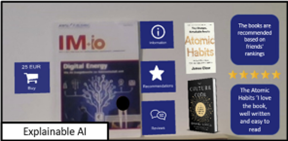
\includegraphics[width=.5\textwidth]{Picture4.png}}% get height
\subfloat[1: RSS vs ARSS (Usefulness)]{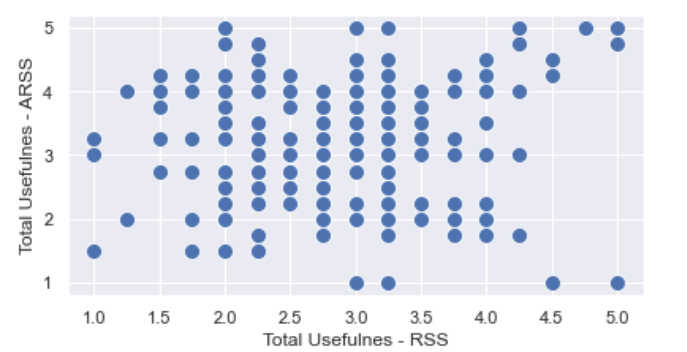
\includegraphics[scale = 0.5]{1.png}}\hfill
\subfloat[2: RSS vs EARSS (Usefulness)]{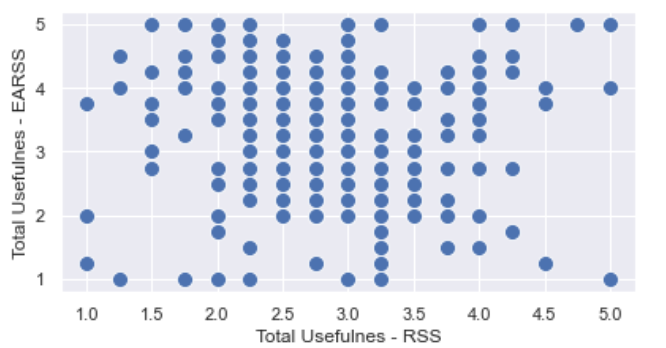
\includegraphics[scale = 0.5]{2.png}}\hfill
\subfloat[3: ARSS vs EARSS (Usefulness)]{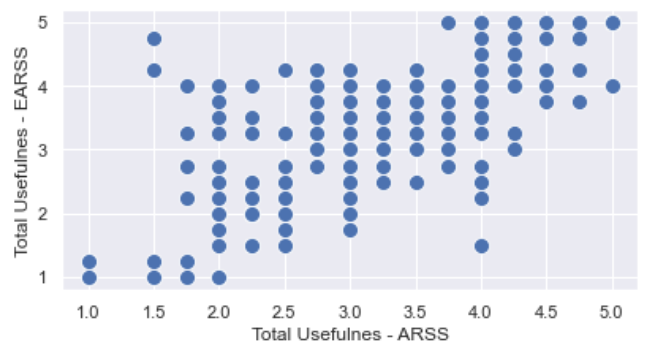
\includegraphics[scale = 0.5]{3.png}}

\end{figure}

\begin{figure}[h!]
The figures(1, 2 and 3) show correlations between RSS, ARSS and EARSS in case of usefulness. as shown in figure (1) and figure (2) there is no linear correlation between them but in figure (3) we can see a strong positive correlation between ARSS and EARSS. 
\end{figure}
\begin{figure}[h!]
The figures (4, 5 and 6) show correlations between RSS, ARSS and EARSS in case of usefulness. as shown in figure (1) and figure (2) there is no linear correlation between them but in figure (3) we can see a strong positive correlation between ARSS and EARSS. 
\end{figure}


\begin{figure}[h!]
\captionsetup[subfigure]{labelformat=empty}
\settoheight{\common}{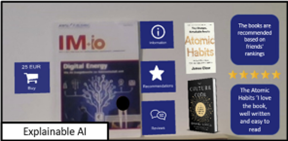
\includegraphics[width=.5\textwidth]{Picture4.png}}% get height
\subfloat[4: RSS vs ARSS (Entertainment)]{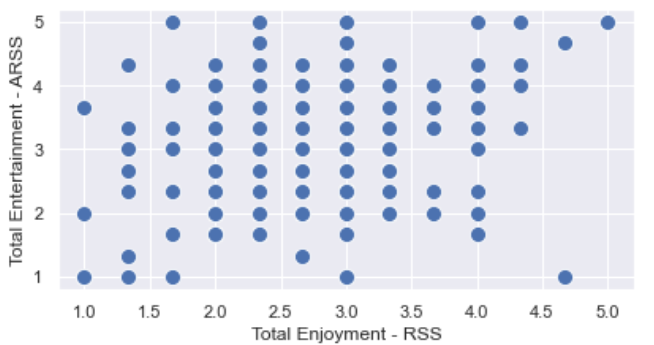
\includegraphics[scale = 0.5]{4.png}}\hfill
\subfloat[5: RSS vs EARSS (Entertainment)]{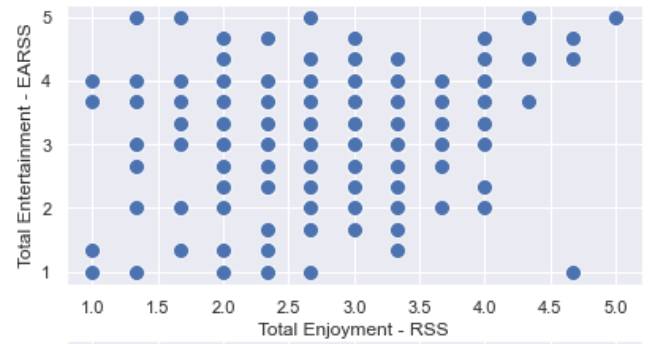
\includegraphics[scale = 0.5]{5.png}}\hfill
\subfloat[6: ARSS vs EARSS (Entertainment)]{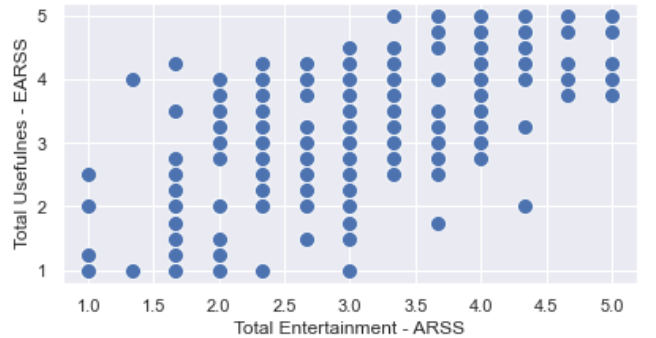
\includegraphics[scale = 0.5]{6.png}}\hfill
\end{figure}

\begin{figure}[h!]
The figures (7, 8 and 9) show correlations between RSS, ARSS and EARSS in case of Informativeness. as shown in figure (8) there is no linear correlation between them but in figure (7 and 9) we can see a strong positive correlation between RSS and EARSS data. 
\end{figure}
\begin{figure}[h!]
The figures (10, 11 and 12) show correlations between RSS, ARSS and EARSS in case of Irritation. as shown in figure (10) and figure (11) there is no correlation between them but in figure (12) we can see a positive correlation between ARSS and EARSS. 
\end{figure}
\begin{figure}[h!]
The figures (13, 14 and 15) show correlations between RSS, ARSS and EARSS in case of Purchase Intention. as shown in figure (14) there is no correlation between them but in figure (15) we can see a strong positive correlation between ARSS and EARSS. meanwhile it is weak on figure (13) between  RSS and ARSS.
\end{figure}
\begin{figure}[h!]
\captionsetup[subfigure]{labelformat=empty}
\settoheight{\common}{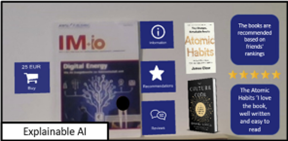
\includegraphics[width=.5\textwidth]{Picture4.png}}% get height
\subfloat[7: RSS vs ARSS (Informativeness)]{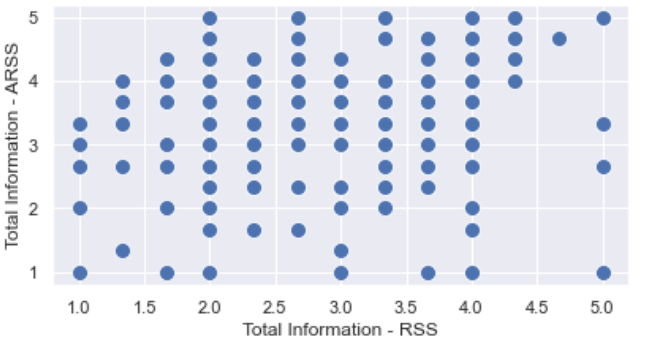
\includegraphics[scale = 0.5]{7.png}}\hfill
\subfloat[8: RSS vs EARSS (Informativeness)]{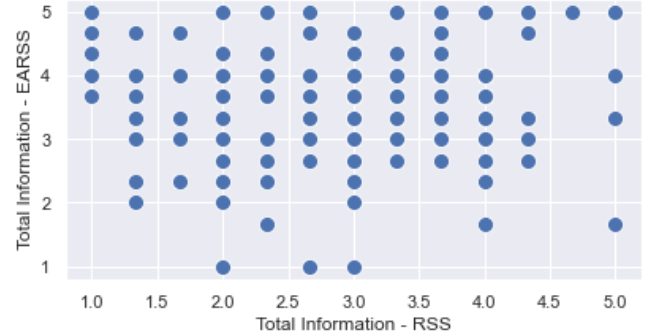
\includegraphics[scale = 0.5]{8.png}}\hfill
\subfloat[9: ARSS vs EARSS (Informativeness)]{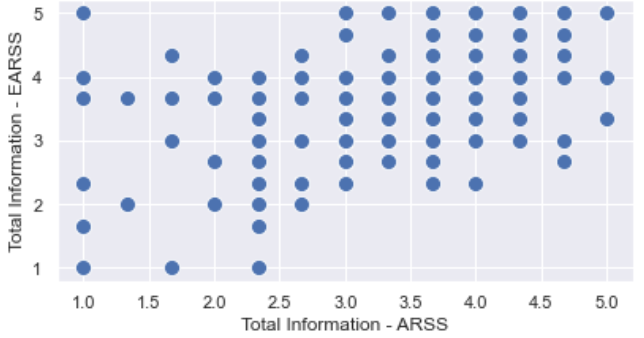
\includegraphics[scale = 0.5]{9.png}}
\end{figure}

\begin{figure}[h!]
In analysing the trust factor between scenarios we would be working only on ARSS and EARSS due to unavailability of data for RSS. as it is shown in figure (16) there is a strong positive correlation between ARSS and EARSS in trust cases.
\end{figure}

\begin{figure}[h!]
\captionsetup[subfigure]{labelformat=empty}
\settoheight{\common}{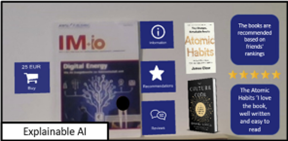
\includegraphics[width=.5\textwidth]{Picture4.png}}% get height
\subfloat[10: RSS vs ARSS (Irritation)]{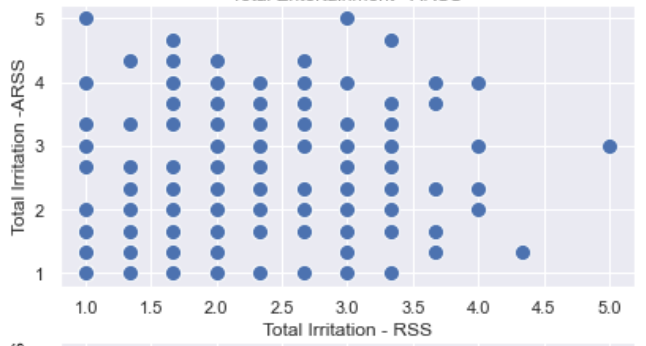
\includegraphics[scale = 0.5]{10.png}}\hfill
\subfloat[11: RSS vs EARSS (Irritation)]{\includegraphics[scale = 0.5]{11.png}}\hfill
\subfloat[12: ARSS vs EARSS (Irritation)]{\includegraphics[scale = 0.5]{12.png}}\hfill
\end{figure}
\begin{figure}[h!]
correlation test does not equal causation. Correlation analysis identities and evaluates a relationship between two variables and a positive correlation does not automatically mean one variable affect the other one. in analysing the results of correlation test in pearsonr and spearman's it is between 1 and -1. it is meant that -1 stands for a perfect negative correlation meanwhile 1 shows a perfect positive and the closer it gets to 0 the strength of correlation is getting weaker respectfully. the main difference between spearman and pearson is that, spearman's correlation is non-parametric meanwhile pearsonr is used for parametric data. furthermore, pearson is a good choice if the data is continuous. alongisde, kendal's tau is used when your data is continous or ordinal and should have monotonic relationship.
\end{figure}
\begin{figure}[h!]
\captionsetup[subfigure]{labelformat=empty}
\settoheight{\common}{\includegraphics[width=.5\textwidth]{Picture4.png}}% get height
\subfloat[13: RSS vs ARSS (Purchase Intention)]{\includegraphics[scale = 0.5]{13.png}}\hfill
\subfloat[14: RSS vs EARSS (Purchase Intention)]{\includegraphics[scale = 0.5]{14.png}}\hfill
\subfloat[15: ARSS vs EARSS (Purchase Intention)]{\includegraphics[scale = 0.5]{15.png}}\hfill
\end{figure}

\begin{figure}[h!]
\captionsetup[subfigure]{labelformat=empty}
\settoheight{\common}{\includegraphics[width=.5\textwidth]{Picture4.png}}% get height
\subfloat[16: ARSS vs EARSS (Trust)]{\includegraphics[scale = 0.5]{16.png}}\hfill
\end{figure}


\begin{figure}[h!]
\subsection{Statistical Tests}
So far we have measured our data in case of curves of distribution and applied different normality tests. Furthermore, we applied different correlation tests to gain an overall idea about our data. According to the results gained from those procedures we have specified our hypothesis. Hypothesis are a supposition or proposed explanation made on the basis of limited evidence as a starting point for further investigation. By measuring the mean of data and standard deviations we have get closed to prove hypothesis but to get to sharp results always statistical tests are required. Statistical tests are divided into two parts. Parametric and non-parametric. 
\\\textbf{Independent t-test:} Used when you want to compare the means of precisely two tests.
\\\textbf{Paired t-test:} Used when we are interested in the difference between two variables for the same subject.
\\\textbf{Anova:} Used when you have collected data about one categorical independent and one quantitative dependent data and it is usually helpful for \\Testing three or more variables.
\\\textbf{RMAnova:} When you have the same measures that the participants were rated on at more than two time points or in other words it is usually used to analyze groups of related dependent variables that represents different measures.
\\\textbf{Mannwhiteneyu:} It is used when data is ordinal or when the assumptions of the t-test are not met.
\\\textbf{Wilcoxon:} it is used whenever you have data that are composed of  definite scores.
\\\textbf{Kruskal:} is used when you have three or more categorical, independent groups.
\\\textbf{Friedman:} It is used to test difference between groups when the dependent variable being measured is ordinal. \\\\

\end{figure}

\begin{table}[h!]
\begin{tabular}{|l|l|l|l|l|}
\hline
             & Scenario     & Paired T-test & Mannwhit. & Wilcoxon \\ \hline
Usefulness   & RSS - ARSS   & 0.000         & 0.00          & 4.588    \\ \hline
             & RSS - EARSS  & 0.000         & 0.00          & 1.678    \\ \hline
             & ARSS - EARSS & 0.005         & 0.08          & 0.008    \\ \hline
Enjoyment    & RSS - ARSS   & 0.000         & 0.00          & 1.300    \\ \hline
             & RSS - EARSS  & 0.000         & 0.00          & 2.799    \\ \hline
             & ARSS - EARSS & 0.141         & 0.31          & 0.075    \\ \hline
Information  & RSS - ARSS   & 0.000         & 0.00          & 7.661    \\ \hline
             & RSS - EARSS  & 0.000         & 0.00          & 1.269    \\ \hline
             & ARSS - EARSS & 0.000         & 0.00          & 2.668    \\ \hline
Irritation   & RSS - ARSS   & 0.000         & 0.01          & 0.001    \\ \hline
             & RSS - EARSS  & 0.002         & 0.03          & 0.009    \\ \hline
             & ARSS - EARSS & 0.637         & 0.72          & 0.700    \\ \hline
P. Intention & RSS - ARSS   & 0.123         & 0.28          & 0.212    \\ \hline
             & RSS - EARSS  & 0.553         & 0.78          & 0.783    \\ \hline
             & ARSS - EARSS & 0.121         & 0.44          & 0.087    \\ \hline
Trust        & RSS - ARSS   & N/A           & N/A           & N/A      \\ \hline
             & RSS - EARSS  & N/A           & N/A           & N/A      \\ \hline
             & ARSS - EARSS & 0.009         & 0.15          & 0.026    \\ \hline
\end{tabular}
\caption{\label{table}Statistical Test Results}
\end{table}
\begin{figure}[h!]
As we previously mentioned the significance value will be (P = 0.05) for all the test in this research. Table [V] is showing the results gained by applying statistical tests needed two groups, meanwhile, table[VI and VII] is the result of tests which needed three groups to compare.
\end{figure}

\begin{table}[h!]
\begin{tabular}{|l|l|l|l|l|}
\hline
             & Scenario           & Kruskal & Friedman & Anova \\ \hline
Usefulness   & RSS - ARSS - EARSS & 6.649   & 1.074    & 4.558 \\ \hline
Enjoyment    & RSS - ARSS - EARSS & 7.938   & 2.438    & 1.300 \\ \hline
Information  & RSS - ARSS - EARSS & 6.525   & 1.536    & 7.661 \\ \hline
Irritation   & RSS - ARSS - EARSS & 0.018   & 0.034    & 0.001 \\ \hline
P. Intention & RSS - ARSS - EARSS & 0.542   & 0.376    & 0.212 \\ \hline
Trust        & RSS - ARSS - EARSS & 0.150   & N/A      & N/A   \\ \hline
\end{tabular}
\caption{\label{table}Statistical Test Results}
\end{table}

\begin{table}[h!]
\begin{tabular}{|m{2.5cm}|m{3.0cm}|m{2.0cm}|}
\hline
             & Scenario           & RMAnova \\ \hline
Usefulness   & RSS - ARSS - EARSS & 3.502   \\ \hline
Enjoyment    & RSS - ARSS - EARSS & 2.110   \\ \hline
Information  & RSS - ARSS - EARSS & 4.078   \\ \hline
Irritation   & RSS - ARSS - EARSS & 0.000   \\ \hline
P. Intention & RSS - ARSS - EARSS & 0.249   \\ \hline
Trust        & RSS - ARSS - EARSS & N/A     \\ \hline
\end{tabular}
\caption{\label{table}Statistical Test Results}
\end{table}

\begin{table}[h!]
\begin{tabular}{|l|l|l|l|l|}
\hline
                & Scenario     & MD     & T-Value & P-Value          \\ \hline
Usefulness      & RSS - ARSS   & -0.367 & -4.758  & \textless{}0.001 \\ \hline
                & RSS - EARSS  & -0.491 & -6.08   & \textless{}0.001 \\ \hline
                & ARSS - EARSS & -0.124 & -1.432  & 0.1516           \\ \hline
Entertainment   & RSS - ARSS   & -0.279 & -3.597  & \textless{}0.001 \\ \hline
                & RSS - EARSS  & -0.350 & -4.436  & \textless{}0.001 \\ \hline
                & ARSS - EARSS & -0.071 & -0.85   & 0.3912           \\ \hline
Informativeness & RSS - ARSS   & -0.429 & -5.27   & \textless{}0.001 \\ \hline
                & RSS - EARSS  & -0.744 & -9.941  & \textless{}0.001 \\ \hline
                & ARSS - EARSS & -0.314 & -4.017  & \textless{}0.001 \\ \hline
Irritation      & RSS - ARSS   & -0.256 & -3.105  & 0.002            \\ \hline
                & RSS - EARSS  & -0.232 & -2.758  & \textless{}0.001 \\ \hline
                & ARSS - EARSS & 0.023  & 0.261   & \textless{}0.001 \\ \hline
Purchase Int.   & RSS - ARSS   & 0.104  & 1.304   & 0.002            \\ \hline
                & RSS - EARSS  & 0.043  & 0.528   & 0.006            \\ \hline
                & ARSS - EARSS & 0.060  & 0.712   & 0.793            \\ \hline
Trust           & RSS - ARSS   & N/A    & N/A     & N/A              \\ \hline
                & RSS - EARSS  & N/A    & N/A     & N/A              \\ \hline
                & ARSS - EARSS & -0.074 & -1.244  & 0.213            \\ \hline
\end{tabular}
\caption{\label{table}Independent T-Test Results}
\end{table}

\begin{figure}[h!]
\textbf{Statistical test results:} Now that we analyzed and applied all tests, we can start accepting or rejecting our hypotheses. Focusing on all tests might be give overlapping answers. hence, we choose tests suitable with distribution of our data. As the result Paired t-test and Anova would be considered to analyze. 
As we hypothesized in h1, h2 and h3 ARSS and EARSS are way much more preferred in terms of Usability, Entertainment and Enjoyment and as the result of the tests we can accept these hypothesis since the significance level received was < 0.05. As in h4 it is also accepted that most of users find RSS much more Irritable than ARSS or EARSS. Here again the significance level received were below 0.05. In h5 we mentioned that ARSS and EARSS are having more intention on user to make them buy products but according to the results we received from the test there is no significant results to accept this hypothesis. H6 was supporting that EARSS is much more trusted than ARSS. The hypothesis is also accepted since the significance level received is 0.009. 

\end{figure}


\begin{figure}[h!]
\subsection{Machine Learning} Machine learning is a branch of artificial intelligence that enables computer systems to learn and improve their abilities through experience without explicit instructions. This is achieved by training the system with a large amount of data, allowing it to make predictions or decisions based on that data. There are various methods for training a machine learning model, including supervised and unsupervised learning. In supervised learning, the model is provided with labeled data, where the correct output for each input is given. On the other hand, in unsupervised learning, the model is not given any labeled data and must find patterns in the data on its own. To have high value predictions which can help to do better decisions listed algorithms are applied.

\textbf{Logistic Regression:} Logistic regression is a type of supervised learning algorithm that is used for classification problems. It is a linear model that is used to predict a binary outcome (i.e., a value of 0 or 1) based on one or more input variables.\\
\textbf{Decision Tree:} A decision tree is a type of machine learning algorithm that is used for both classification and regression tasks. It is a flowchart-like tree structure that makes decisions based on the value of an attribute in the input data.\\
\textbf{K Neighbors:} k-nearest neighbors (k-NN) is a type of supervised learning algorithm that is used for both classification and regression tasks. It is a non-parametric method, which means that it does not make any assumptions about the underlying data distribution.\\
\textbf{Support Vector Machine:} Support vector machine (SVM) is a type of supervised learning algorithm that is used for both classification and regression tasks. It is a linear model that is used to find the hyperplane in a high-dimensional space that maximally separates the classes in a dataset.\\
\textbf{Random Forrest:} Is a type of supervised learning algorithm that is used for both classification and regression tasks. It is an ensemble method, which means that it combines the predictions of multiple models to improve the overall performance.
\end{figure}




\begin{table}[h!]
\begin{tabular}{|l|l|l|l|l|l|}
\hline
           & Log. R. & Dec. T. & K. Neighbors & SVM   & Random F. \\ \hline
Train Acc. & 0.636       & 1.00        & 0.664       & 0.630 & 0.994     \\ \hline
Test Acc.  & 0.631       & 0.434       & 0.539       & 0.631 & 0.447     \\ \hline
F1 Score   & 0.631       & 0.434       & 0.539       & 0.631 & 0.447     \\ \hline
C. Val.   & 0.91       & 0.77       & 0.87       & 0.94 & 0.89     \\ \hline
\end{tabular}
\caption{\label{table}RSS Machine Learning Results}
\end{table}

\begin{table}[h!]
\begin{tabular}{|l|l|l|l|l|l|}
\hline
           & Log. R. & Dec. T. & K Neighbors & SVM   & Random F. \\ \hline
Train Acc. & 0.647       & 1.00        & 0.647       & 0.647 & 1.00      \\ \hline
Test Acc.  & 0.644       & 0.447       & 0.513       & 0.644 & 0.447     \\ \hline
F1 Score   & 0.644       & 0.447       & 0.513       & 0.644 & 0.447     \\ \hline
C. Val.   & 0.90       & 0.78       & 0.87       & 0.92 & 0.87     \\ \hline
\end{tabular}
\caption{\label{table}ARSS Machine Learning Results}
\end{table}

\begin{table}[]
\begin{tabular}{|l|l|l|l|l|l|}
\hline
           & Log. R. & Dec. T. & K Neighbors & SVM   & Random F. \\ \hline
Train Acc. & 0.602       & 1.00        & 0.670       & 0.602 & 0.994     \\ \hline
Test Acc.  & 0.605       & 0.421       & 0.500       & 0.605 & 0.407     \\ \hline
F1 Score   & 0.605       & 0.421       & 0.500       & 0.605 & 0.407     \\ \hline
C. Val.   & 0.85       & 0.83       & 0.85       & 0.92 & 0.87     \\ \hline
\end{tabular}
\caption{\label{table}EARSS Machine Learning Results}
\end{table}




\begin{figure}
But before jumping to all these algorithms we have to select and split our train and test data. In this case, I decided to generate a separate dataset for the third of scenarios and rewrite columns regarding to each scenario. Next, I assigned all of them as train data and wanted to make predictions separately on each of three scenarios as shown in table [table numbers]. It is good to underline that I separated 70\% of data for training and 30\% for testing. 
In case to use sampling, since the dataset were already small and applying sampling method was risky due to losing or not appearing some values; It has been decided to implement data without applying any sampling methods. \\
As it is shown in Tables [[IX, X, XI]] the accuracies are not satisfying, hence, it is decided to apply different methods to increase the accuracy. As first steps I applied different algorithms, but the results were pretty close to the ones already taken. I changed the train test parameters and values but it was still same. As the last step I tried to apply cross validation and the results were satisfyingly good as mentioned in Tables [IX, X, XI] regarding to each scenario.



\subsection{Text Analysis}
At the end of the survey, the participants were asked 8 different questions. In this part of the survey they were not supposed to answer by grading them but this time, it was requested to explain there thoughts. \\
At the beginning it looked like a good idea to apply some sentiment analysis algorithms but there was nothing asked regarding to their feelings or anything to make them to express their feelings. \\
In this case, before starting the procedure to make out certain information some preprocessing methods are also done. Dropping the stop-word from the sentences, dropping special symbols and number, Dropping double spaces and lower casing the words are among the methods applied.
While analysis of these questions I  decided to start with tearing sentences into N-words. In this method the algorithm developed was accountable to outline the compounded words which was taking us to the main ideas of participants by separating them into two and three gram words which is helpful to reach to the main idea of the sentences written.\\\\
The questions asked are listed below:


1. Are there any feature missing?\\
2. Do you see any issue or room to improve?\\
3. Would it help you during Covid-19?\\
4. Would it motivate you to shop-in-store?\\
5. Did you find the app explanations helpful?\\
6. In shopping of what would you like t use?\\
7. Are you satisfied with Brick-and-mortar?\\
8. What technologies should be provided?\\


\end{figure}
\begin{figure}[h!]
\begin{enumerate}
  \item The result of N-word for first question which was asking about missing features of the application is listed below: “Comparison Shops”, “Shops Near Environment”, “Ingredients of product”, “Shopping List”, “Prices”, “Misspelling Augmented” and most of the rest were complements about the application.\\
  \item Second question was regarding to improvement of issues. Mostly used compound word here was “Shopping List”, “Scanning Products”, ”Alternative Products”, ”Data Privacy”, ”Unattractive Design”, ”Lack Balance” and etc.\\
  \item In this part participants were asked that to review the pros and cons of this concept during covid-19. To share in them respectively Most of them said “don’t know”, “Yes” and “No”. meanwhile some of them was preferring “Online Shopping”.\\
  \item The fourth question was asked to know if this concept is motivating participants to buy things. Surprisingly a huge amount of them was responding positive and mentioning “Having Fun” while using this concept. Meanwhile, some of them was concerning about “Spending Time” and lack of “Product Information”.\\
  \item This Question was asked to know if the given information by application was satisfying enough or not. From the compound compiled we noticed that most of them were shown satisfied basically but also requesting for detailed information of Products.\\
  \item The sixth question was about to know in which fields this technology must be used in. The answers coming from participants were “Electronics”, ”Clothing”, ”Food Products”. In conclusion huge amount of them wanted on electronic and clothing items.\\
  \item Here it was asked to know that the participants were satisfied with brick-and-mortar services so far. And frankly, A huge amount of them was answered positively. And it is good to know that no negative answer compiled by our code.\\
  \item As the last question of survey, they asked for technologies must be provided, the answers were creative. “Digital Shopping”, “Online Shopping”, “Virtual Reality”, “Trying Clothes On”, “Robots Services” “Delivery services”, “Electronic pay”, “Scanned codes” and “Providing information” were among the answers.\\


\end{enumerate}
\end{figure}


\begin{figure}[h!]
\section{CONCLUSIONS}
Technology is the most effective field in case to help mankind to achieve comfort and be able to live in a best way possible. The attempts done in this field are uncountable. One of those attempts is Augmented Reality. Recently it is contributing to any part of our lives from education to entertainment but this document contained the idea of using augmented reality and artificial intelligence in shopping industry. Developing such ideas without being assure if it is accepted by users or not, might be risky from different perspectives. Therefore, in case to prevent such risks suppliers share a demo or ask the customers ideas through surveys. This research was analyzing the results of a survey. The goal was to compare three different shopping scenarios. Respectively, Regular Shopping Scenarios, Augmented Reality Shopping Scenario and Explainable Artificial Intelligence Augmented Reality Shopping Scenario. Participants asked from different fields like, usefulness, entertainment, informativeness, irritation, shopping intention and trust factor between these three scenarios. After introducing the concepts, the research started with analyzing and getting to know the participants. chart and tables [Chart and table numbers] are visualized summarize of participants analyzed from as many different aspects as possible. There are also 8 questions which was asked the ideas of customers regarding to these scenarios. This research also contains text analysis of those fields, which can lead us to some really good results. The main part of research was to compare the shopping scenarios. The comparing done and proved by Independent T-test and measured through different values. The results were pointing that ARSS and EARSS is more useful, entertainable, informative. Most of them found RSS irritable than ARSS and EARSS. The purchase intention of RSS was higher than ARSS and EARSS. Finally in case being trustful EARSS has a high range than ARSS. As in any other research this research also had its limitations. The amount of participants were not satisfyingly high therefore, the results might not be accurate to decide but is perfectly good to take first steps according to it. 

\begin{thebibliography}{99}


\bibitem{c1} Verhoef, P.C., Kannan, P.K. and Inman, J.J. (2015), “From multi-channel retailing to omni-channel
retailing. Introduction to the special issue on multi-channel retailing”, Journal of Retailing,
Vol. 91 No. 2, pp. 174-181, doi: 10.1016/j.jretai.2015.02.005.
\bibitem{c2} Lavoye, V., Mero, J. and Tarkiainen, A. (2021), “Consumer behavior with augmented reality in retail: a
review and research agenda”, The International Review of Retail, Distribution and Consumer
Research, Vol. 31 No. 3, pp. 299-329, doi: 10.1080/09593969.2021.1901765.
\bibitem{c3} Parise, S., Guinan, P.J. and Kafka, R. (2016), “Solving the Crisis of Immediacy: how digital technology
can transform the customer experience”, Business Horizons, Vol. 59 No. 4, pp. 411-420, doi: 10.
1016/j.bushor.2016.03.004.
\bibitem{c4} Nasibullah Qarizada, (2022), "The impacts of Covid-19 on Education"
\bibitem{c5} https://www.kaggle.com/code/sudalairajkumar/an-interactive-deep-dive-into-survey-results/notebook
\bibitem{c6} Robert Zimmermann, Daniel Mora, Douglas Cirqueira (2021), "Enhancing brick-and-mortar store shopping experience with an
augmented reality shopping assistant application using personalized recommendations and explainable artificial intelligence"

\end{thebibliography}
\end{figure}
\end{document}
